\documentclass[letterpaper]{article}

% !TEX root = paper.tex

\usepackage{algorithm}
\usepackage{algpseudocode}
\usepackage{amsmath}
\usepackage{amssymb}
\usepackage{amsthm}
\usepackage[titletoc]{appendix}
\usepackage{array}
\usepackage[english]{babel}
\usepackage{cancel}
\usepackage{color}
\usepackage{eqparbox}
\usepackage{float}
\usepackage[T1]{fontenc}
\usepackage{graphicx}
\usepackage[hidelinks]{hyperref}
\usepackage[utf8]{inputenc}
\usepackage{lipsum}
\usepackage{microtype}      % microtypography
\usepackage[cache=false]{minted}
\usepackage{nicefrac}       % compact symbols for 1/2, etc.
\usepackage{pgfplots}
\usepackage{scalerel}
\usepackage{skull}
\usepackage{subcaption}
\usepackage{titling}
\usepackage{textcomp}
\usepackage{tikz}
\usepackage{tikz-3dplot}
\usepackage{textcomp}
\usepackage[nottoc]{tocbibind}
\usepackage[textsize=small]{todonotes}
\usepackage[normalem]{ulem}
\usepackage{wrapfig}

% Settings
\definecolor{__minted_background_color}{rgb}{0.95, 0.95, 0.98}
\definecolor{__minted_highlight_color}{rgb}{0.88, 0.88, 1.0}
\setminted{autogobble=true,
           style=tango,
           breaklines,
           bgcolor=__minted_background_color,
           highlightcolor=__minted_highlight_color,
           % mathescape, % Escape math mode everywhere, not needed with the following.
           texcomments,  % Enable latex code inside of comments. Useful for referencing equations.
    }
\pgfplotsset{compat=1.15}
\usetikzlibrary{decorations.pathreplacing}

% Definitions

% Blackboard hacks because NIPS can't do real fonts...
\newcommand{\R}{I\!\!R}     % real numbers
\newcommand{\N}{I\!\!N}     % natural numbers
\newcommand{\C}{I\!\!\!\!C} % complex numbers

% An inline TODO command
\newcommand\todoinline[2][]{\todo[inline, caption={TODO}, #1]{
    \begin{minipage}{\textwidth-4pt}#2\end{minipage}}}

% Load nips_2017 last to override any changes I didn't mean to make.
\usepackage[final]{nips_2017}

\title{Generating presidential tweets with an LSTM network}

\author{%
    Austin Gill\\
    Department of Mathematics and Computer Science\\
    South Dakota School of Mines and Technology\\
    Rapid City SD, 57701\\
    \texttt{\href{mailto:austin.gill@mines.sdsmt.edu}{austin.gill@mines.sdsmt.edu}}\\
}

\begin{document}
\maketitle

\begin{abstract}
    We motivate and develop a recurrent generational model to generate tweets similar to those of President Donald J. Trump. We outline previous research in generational models, and point out the difficulties of objective measurement of inherently subjective creative models. After experimenting with several recurrent models, we settle on a 6 layer, 64 unit LSTM model, and recommend a more advanced model as proposed by other research. We finally recommend using advanced natural language processing techniques to develop a Generative Adversarial Network in any future work.
\end{abstract}

\section{Introduction}
    The field of classifying text with machine learning models is well-studied. However, the field of text-generational models is still being actively researched. Generational models are interesting because there is no true idea of ``accuracy'' because the models are \textit{creative}. Given some input, a generational model does not seek to produce an output identical to that of the training set. Instead, there is a subtle tug-of-war between reproducing text samples found in the training set and producing \textit{new} text samples that sound similar.

    The author's original goal was to produce a machine learning model to generate haikus, a short form of Japanese poetry. \citet{yael_2010} used word association norms to extend previous generational models to generate haikus with some success. However, the author was unable to scrape together a large enough data set to build a model. Additionally, \citet{yael_2010} did not specify their model architecture in detail, leaving more research to be done than the author had time for.

    However, there have been a number of open source implementations of generational models for larger pieces of text. \citet{thoutt_2017} built a generational model to generate the sixth \textit{A Song of Ice and Fire} \citep{martin} book due to its untimely publication.

    Finding an interesting and relevant text generation problem with a large corpus to train a model on was as easy as turning to Twitter. There has been recent research using Twitter. \citet{felbo_2017} produced a model to perform sentiment, emotion, and sarcasm analysis on tweets taking into account their use of Emoji characters. \citet{woolf_2017} constructed a sophisticated model to generate similar-sounding tweets. However, \citet{woolf_2017} also attempted (with success) to train on the tweets of multiple Twitter users, and used contextual tagging to generate tweets combining the semantics of multiple (and possibly quite differently behaving) users. Twitter provides a fairly simple API to download a user's tweets. However, the API limits the number tweets available to the 3200 most recent tweets. This was a smaller data set than the haikus the author was able to scrape together.

    Luckily we live in a time where passionate people can put an extraordinary amount of effort in building a publicly accessible archive of tweets by prominent politicians. \citet{brown_2017} produced a public archive of President Donald J. Trump's tweets and hosted it on GitHub for public use. The archive is updated hourly, and does to remove deleted tweets.

    Before deep learning's rise to fame, text generation was done using probabilistic Markov models where the next word in a sequence was generated based on the current (and only the current) state in the Markov chain. These models lacked enough context to construct cogent text samples reliably. Recurrent machine learning models are the current response to providing contextual information.

    Rather than generate the next token in a sequence based only on the previous token, recurrent models provide some amount of history so that the training can pick up on larger patterns in the training data, typically referred to as the corpus when dealing with text. \citet{karpathy_2015} has done quite a bit of research using recurrent models with a generational purpose. For example, \citet{karpathy_2015} constructed recurrent models trained on the Linux kernel source code, as well as various mathematical research papers, to produce various C and \LaTeX{} code that almost compiled!

    The current standard model in text generational models, according to \citet{karpathy_2015}, is some number of Long Short-Term Memory (LSTM) layers followed by a single densely connected output layer with a softmax activation function to provide a one-hot token encoding vector as an output.

    As mentioned though, accuracy does not make a useful metric to monitor training progression because generational models do not seek to reproduce the training set. Instead, they attempt to produce a new corpus that has some amount of similarity. In scope, the author did not have the resources to provide an in-depth similarity analysis, and instead relied on a subjective personal measure of how well the produced models performed.

\section{Experiments}
    \subsection{Inspiration}
        Most heavily, the author was inspired by previous work generating large corpuses by \citet{thoutt_2017} and the work on recurrent architectures by \citet{karpathy_2015}. In short, the author chose to deal almost exclusively with LSTM layers in some configuration with a one-hot encoded softmax output.

        Due to ease-of-use and a simple high-level interface, the author chose to implement all models using Keras \citep{chollet2015keras}. Keras provided an acceptably abstracted view of the models that enabled to author to focus on the model architecture rather than each model's implementation.

    \subsection{Data Formatting}
        After retrieving the tweets from \citet{brown_2017}'s archive, the next difficulty was deciding how to effectively format the data to facilitate its use in a neural network. Based on the Keras documentation and LSTM generational examples, the author decided to follow the following three steps

        \begin{figure}[H]
            \centering
            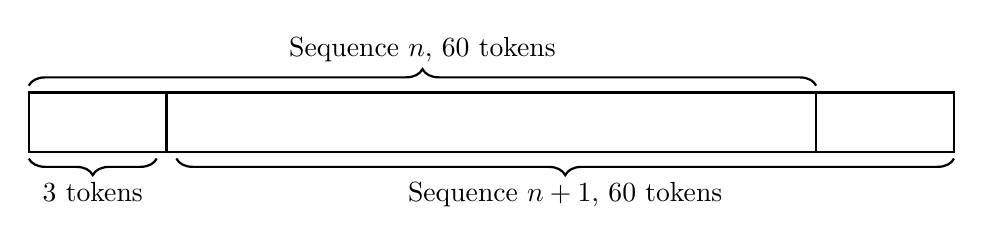
\begin{tikzpicture}[scale=0.25]

                \draw[thick] (0, 0) rectangle (40, 3);
                \draw[thick] (7, 0) rectangle (47, 3);
                \draw [decorate,
                       thick,
                       decoration={brace, amplitude=6pt, mirror},
                       xshift=0pt,
                       yshift=-10pt]
                    (0, 0) -- node[midway, below, yshift=-5] {3 tokens} (6.5, 0);
                \draw [decorate,
                       thick,
                       decoration={brace, amplitude=6pt},
                       xshift=0pt,
                       yshift=10pt]
                    (0, 3) -- node[midway, above, yshift=5] {Sequence $n$, 60 tokens} (40, 3);
                \draw [decorate,
                       thick,
                       decoration={brace, amplitude=6pt, mirror},
                       xshift=0pt,
                       yshift=-10pt]
                 (7.5, 0) -- node[midway, below, yshift=-5] {Sequence $n + 1$, 60 tokens} (47, 0);
            \end{tikzpicture}
            \caption{Chunking the corpus into overlapping sequences}\label{fig:sequences}
        \end{figure}

        \begin{enumerate}
            \item Preprocess the data to remove Emojis, retweets, capitalization, URLs, images, etc.

            Other tweet generation projects remove username ``\texttt{@mentions}'' from their training set, but the author felt it was valuable to not strip them out.

            \item Concatenate each tweet to form a larger corpus to sample from.
            \item Chunk the corpus into overlapping sequences of tokens. This forms the inputs to the network. The expected output is the token immediately following the end of each sequence. Each sequence was 60 tokens long and separated by 3 tokens as shown in~\autoref{fig:sequences}
            \item Vectorize each sequence by mapping each token to a vector with a \texttt{TRUE} value in the index corresponding to that token.
        \end{enumerate}

        % I have a new hatred for floating wrapped figures. Welcome to a new kind of hell.
        % Also, tall and skinny figures just aren't a good idea...
        \begin{wrapfigure}[47]{r}[40pt]{0pt}
            \centering
            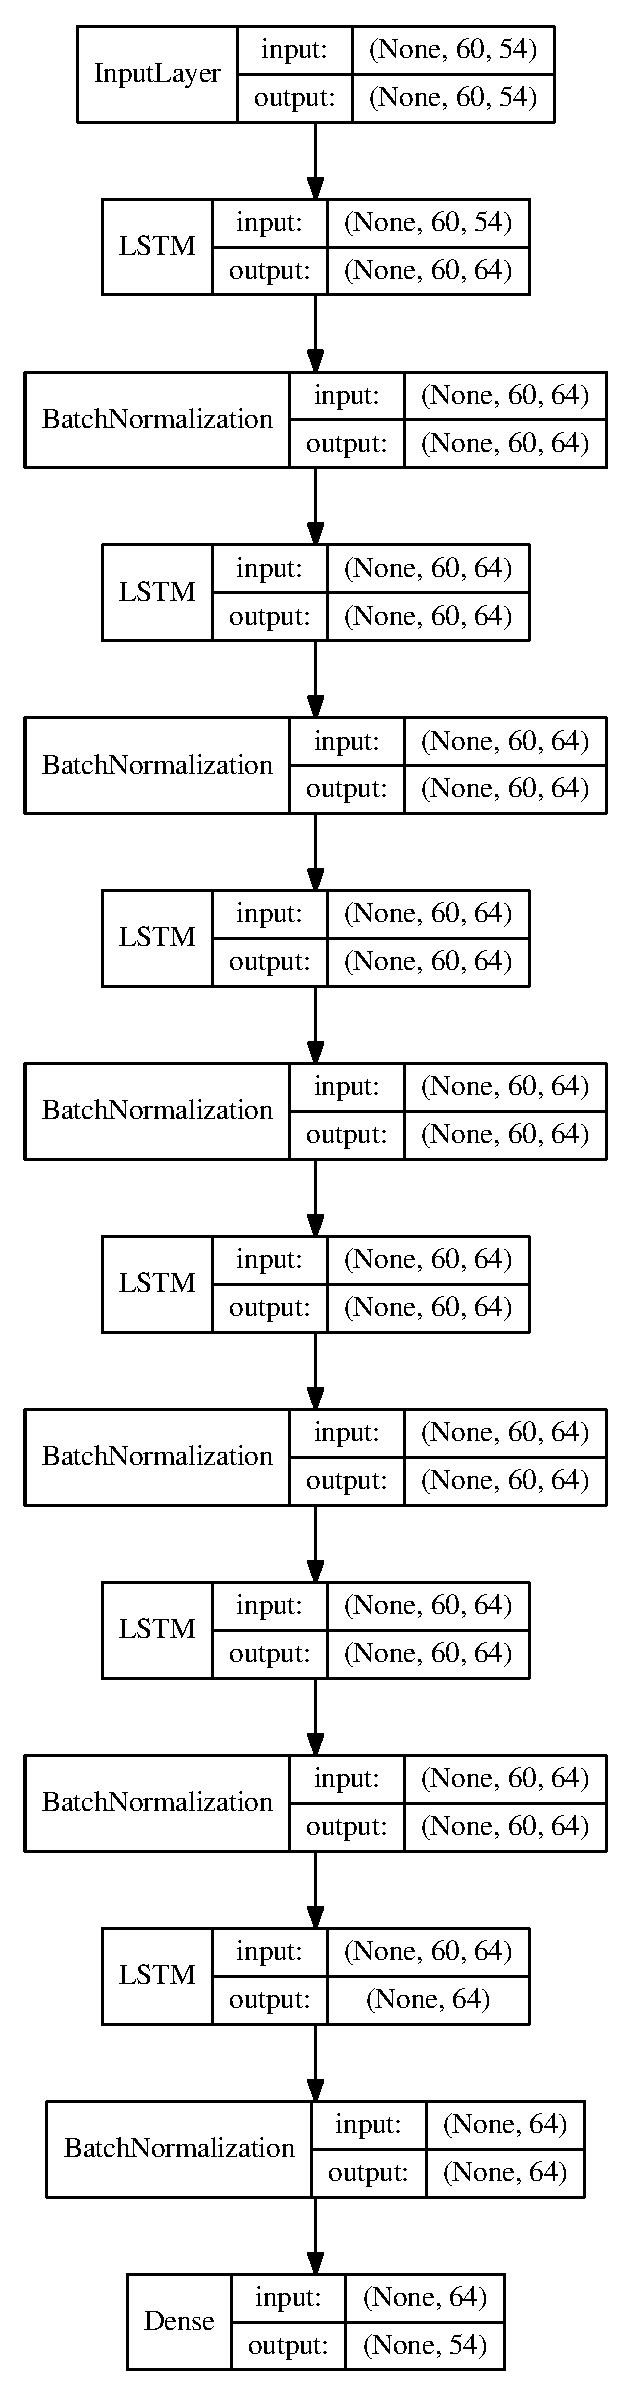
\includegraphics[width=0.36\textwidth]{figures/64x6.eps}
            \caption{A deep and narrow LSTM model using batch normalization}\label{fig:architecture-64x6}
        \end{wrapfigure}

        There are two options for tokenizing the corpus. The author chose to tokenize by character rather than by word. This means that the vectorized sequences are sequences of characters, and the model is predicting the very next character of each sequence.

        Additionally, the sequences overlap a great deal, and contain an enormous amount of redundant data. The dataset in JSON form takes a mere 9.3 megabytes, but in vectorized form takes almost 5 gigabytes. Also note that even though there are only $\sim 37$ thousand tweets by President Trump, the vectorized dataset turns into $\sim 1.1$ \textit{million} sequences.

        Also note that the author trained the experimental models on \textit{all} of President Trump's tweets from his account creation in 2009 to 2018.

    \subsection{Model Architectures}
        The author attempted 21 different variations of LSTM models in both height and depth. Most examples and online recommendations were to use relatively shallow networks with height determined by circumstance.

        One such configuration that showed promise is shown in~\autoref{fig:architecture-64x6}. This model was composed of six 64-unit LSTM layers with batch normalization. Each configuration used 60 character long sequences as the model input, and a one-hot encoded vector output to indicate the most likely next character in the sequence.

        While the author experimented with regularization, overfitting was not an issue due to the sheer size of the training set. Thus, most of the best performing models used batch normalization rather than some form of dropout.

        Note that the author was not able to significantly outperform his first attempt, which consisted of a single 256-unit LSTM layer without batch normalization or dropout.

    \subsection{Training Variations}
        The author initially used the Root Mean Square Propagation (RMSProp) optimization algorithm on recommendation, but also experimented with Stochastic Gradient Decent (SGD) optimizer. RMSProp is an adaptive optimizer that tunes its learning rate as it runs. The author favors RMSProp due to a considerably faster training time in both time elapsed and number of epochs necessary when compared with SGD.

        When using RMSProp, it was typically only necessary to train for around 5 epochs, depending on the model size, while SGD (even with a higher learning rate) took on average 100 epochs to get comparable results. All attempts used a categorical cross-entropy loss function due to the network output being one-hot encoded.

    \subsection{Generating New Tweets}
        The neural network takes in a sequence of the training set, and predicts the next token in the corpus. To take a trained network and generate new tweets, we first begin with a seed randomly taken from the corpus. The network predicts the next token in the sequence as an array of probabilities, which is then sampled with some diversity because the intent of the model is to generate new creative work not found in the training set.

        The newly generated token is appended to the seed, which is then shifted down one token. The author chose to repeat this process until the generated portion of the text (excluding the seed) is 280 characters long.

        This process is repeated using several different probability sampling diversities for each randomly chosen seed, resulting in a different piece of generated text for each diversity. The higher the diversity, the more creative the model became, but at the cost of becoming less and less intelligible. The lower the diversity, the more intelligible became, but at the cost of simply repeating portions of text appearing in the corpus.

\section{Results}
    The results for a few select architectures are summarized below.

    \subsection{256 Unit, 1 Layer LSTM}
        \autoref{fig:256-loss} shows the training loss over time for a basic one-layer 256 unit LSTM model. The author used validation data to get a sense of how well the models generalized. The author did \textit{not} use a test set to evaluate how the model performed at the end of training because of the problem nature. Generational models are not intended to accurately map the training inputs to the training outputs. Thus evaluating the model accuracy on an unseen dataset gives no useful information.

        \begin{figure}[h]
            \centering
            \includegraphics[width=0.7\textwidth]{figures/256dropout20.png}
            \caption{Basic 256 unit LSTM model}\label{fig:256-loss}
        \end{figure}

        Instead, the author used subjective measures to evaluate whether a model performed well or not. The output of this network, for lower sampling diversities, was quite intelligible. Several generated tweets have been cherry-picked, as \citet{karpathy_2015} notes is necessary for recurrent generational models, and shown below.

        Note that all capitalization has been done by hand to make the results more legible.

        \begin{quote}
            ``The debate to the worst and the worst President Obama was a great president of the world is a great person. The Republicans will be a great job on the world''

            ``The state of the state of the world is a great person. The Republicans will be on the world is a great poll to be the best interview discussing the Trump Tower''

            ``@realDonaldTrump is the only one of the worst president of the world is a great person. The Republicans will be a great president of the world''

            ``I have a great people of the worst and the debate to the worst President Obama is a great person. The Democrats are all talk about me to be the best interview discussing the Trump Tower''

            ``The poor for their presidential party of his presidency to start doing for millions of the conservative and brand who has got a state of the good country! We need a state who says Hillary she are an amazing''
        \end{quote}

        It is quite evident that the network is catching on to certain speech patterns, but is completely blind to grammar, and only strings together cogent thoughts over small stretches of the generated text. When considering the sentence structure as a whole, it lacks meaning, but certain substrings (e.g., ``the worst President Obama was a great president'', or ``The Democrats are all talk about me'') form coherent thoughts.

    \subsection{64 Unit, 6 Layer LSTM}
        The following results are using the model shown in \autoref{fig:architecture-64x6}. Note that \autoref{fig:64x6-loss} shows that this model took more training time to reach the same behavior as shown in \autoref{fig:256-loss}. This is expected because it's a larger model.

        \begin{figure}[h]
            \centering
            \includegraphics[width=0.7\textwidth]{figures/64x6-rms-batchnorm-50.png}
            \caption{64 unit, 6 layer LSTM model with batch normalization}\label{fig:64x6-loss}
        \end{figure}

        Again, several cherry-picked tweets are given below with capitalization added.

        \begin{quote}
            ``@MittRomney should be the only one who need it. Good move for the Scott exciting to Russia on @FoxNews for the administration policies commissioner''

            ``Dems is a total loser with the Trump country is a great guy to the great states of The Apprentice''

            ``@BarackObama scandaled will be Donald Trump liars will be a game on @foxandfriends at Americans and winner!''

            ``Bad interview to the Trump country is the states of the first story and states of the Trump International Hotel in the country will be interviewed on @FoxNews and never win in the presidential''

            ``Statements are something to be a truly great guy to the only one who can speak at the Trump Tower to see the president of the US''

            ``Trump country is a great president of the USA and the art of the Democrats are something to be a great support the Trump Tower to make America great again!''

            ``The end of Monday at your cards classing a billionaire inspiration''

            ``And the Trump country is a great president of the USA and the Trump signing to stop president of the USA and the Trump signing to stop and the Trump signitictor is a great president of the USA and states and states of the Trump country is a great president of the USA''
        \end{quote}

    \subsection{1024 Unit, 1 Layer LSTM}
        During the experimentation process, it seemed like the shallow layers produced the most intelligible results, so the author experimented by making the models much much wider. However, the results were not promising. \autoref{fig:1024-loss} shows the training loss over time, which shows that the optimizer struggled with such a large model. Further, training even for 20 epochs took almost 24 hours on an NVIDA GTX 1080.

        \begin{figure}[h]
            \centering
            \includegraphics[width=0.7\textwidth]{figures/1024-rms-batchnorm-20.png}
            \caption{1024 unit LSTM model with batch normalization}\label{fig:1024-loss}
        \end{figure}

        The generated results are given below.

        \begin{quote}
            ``and and and and and and and the and and and and and the and and the and and and and and and and and and and and and and the and and and the and the and the and and the and and the and and and the and and and and and and the and the and than the and and the and and and and and''

            ``@realDonaldTrump i we aa seare to need a fight and and any every is a tered beanies and the of the real in the life and that I live a great and leader I love to the beal about is any and and the me. The thanes and that I and and and lime''

            ``America get I and the thang is and the ane that I at see any I and than Obama in is and peolle last is than the antary this peesident a. The unition so to thanised is a taine in the really and it in I've any way a deal to the for the aldonal and was and we will be a like''
        \end{quote}

    \subsection{Textgenrnn}
        After it was too late to incorporate any meaningful changes, the author was directed to a GitHub project \citep{woolf_2017} built expressly for generating text using a recurrent network. The model architecture is shown in \autoref{fig:architecture-textgenrnn}. This architecture is interesting because it has a context input to allow mixing tagging different pieces of the training set with context. The example usage given in the documentation indicates that this works well when combining text written by different authors.

        \begin{figure}[h]
            \centering
            \includegraphics[width=\textwidth]{figures/context_model.png}
            \caption{Textgenrnn architecture}\label{fig:architecture-textgenrnn}
        \end{figure}

        For completeness, Textgenrnn, as trained by the author, may be used as follows

        \begin{minted}{python}
            from textgenrnn.textgenrnn import textgenrnn  # Installable with Pip
            # Files found in trumperator/experiments/
            t = textgenrnn(config_path='trumperator_config.json',
                           vocab_path='trumperator_vocab.json',
                           weights_path='trumperator_weights.hdf5')
            t.generate(1, temperature=0.2)
        \end{minted}

        Textgenrnn has the option of tokenizing on either words or characters. The following generated samples were created using character-tokenized sequences. Note that any capitalization is \textit{not} added by the author---it was generated by the model. Also note that the documentation stated to train the model for a mere five epochs.

        \begin{quote}
            ``@realDonaldTrump you would be a clue and it's a great season. The Second and a state and all why are you all there, a real estate of him right on his interests and entertaining the U.S. and the world and the great policies are a fantastic game!''

            ``I will be on @foxandfriends at: A.M. Enjoy!''

            ``The Trade Resort is killing our country picks at the borders that we can energy the president of a total leader and a winner of the most broke our since I all television clifful in the other politics of the borders are a great complete disaster.''

            ``@realDonaldTrump the many of the Republican candidates and have been a big problem. \#Trump''

            ``@realDonaldTrump @FoxNews  You are the only one that are with your badly because you support it. The man at our country will be great to have the mother is one of the big millions of comments are looking like a big people of the U.S. he will be so much more than he is the U.S.''

            ``Highly improvement on back with Democrats of the coming evenings than the lands showication and one of the place tomorrow at: A.M.  Enjoy!''
        \end{quote}

        These results seem to be more coherent, but it does seem like it simply strings together substrings from the larger corpus.

\section{Discussion}
    Even taking the entirety of President Trump's tweets (including time not spent in office), cherry-picked results have a quite political flavor. This was unexpected, but welcome as it exacerbated the patterns shown in the generated corpus. Even so, it is difficult to get a good objective grasp of how well generational models perform due to the qualitative nature of their outputs. Therefore, accuracy analysis is essentially meaningless, especially because the intent of generational models is to \textit{avoid} exactly replicating instances in the training set.

    We ultimately recommend using the six-layer, 64 unit LSTM network illustrated in \autoref{fig:architecture-64x6} because the generated output seemed to be more diverse, with less repetition. However, we do have recommendations for future work in this area. There has been an enormous amount of recent research in natural language understanding using machine learning models. The author suggest any further research look into using spaCy \citep{spacy2} to strip each word to its root form, perform part-of-speech tagging, grammar analysis, word association analysis, and other linguistic analysis as a one or more components of a Generative Adversarial Network (GAN).

    The best performing models as a whole generated fairly reasonable results, but as \citet{karpathy_2015} notes, most recurrent generational models produce results that must be scraped by hand to find the best results. We recommend a different strategy for future work however. It seems like the Textgenrnn model could be used as the generative portion of a Generative Adversarial Network, and use some kind of grammar metric as the adversarial component of the model.

    Further, the author also suggests tokenizing at a word level so that the recurrent model predicts the next word in a sequence rather than the next character. This is drastically increase the size of the output vector, but will diminish the size of dataset. It will probably be necessary to prune out the least common words, as well as treat punctuation as individual tokens.

    It would also be possible, if training time is not an issue, to crowd-source the adversarial component of a GAN by tweeting each generated tweet, and recording how many likes or retweets each received.

% Have to use one of the natbib styles. They all suck...
\bibliographystyle{abbrvnat}
% Automatically places a \section*{References}...
\bibliography{paper}
\end{document}
